%% bare_conf.tex
%% V1.3
%% 2007/01/11
%% by Michael Shell
%% See:
%% http://www.michaelshell.org/
%% for current contact information.
%%
%% This is a skeleton file demonstrating the use of IEEEtran.cls
%% (requires IEEEtran.cls version 1.7 or later) with an IEEE conference paper.
%%
%% Support sites:
%% http://www.michaelshell.org/tex/ieeetran/
%% http://www.ctan.org/tex-archive/macros/latex/contrib/IEEEtran/
%% and
%% http://www.ieee.org/

%%*************************************************************************
%% Legal Notice:
%% This code is offered as-is without any warranty either expressed or
%% implied; without even the implied warranty of MERCHANTABILITY or
%% FITNESS FOR A PARTICULAR PURPOSE!
%% User assumes all risk.
%% In no event shall IEEE or any contributor to this code be liable for
%% any damages or losses, including, but not limited to, incidental,
%% consequential, or any other damages, resulting from the use or misuse
%% of any information contained here.
%%
%% All comments are the opinions of their respective authors and are not
%% necessarily endorsed by the IEEE.
%%
%% This work is distributed under the LaTeX Project Public License (LPPL)
%% ( http://www.latex-project.org/ ) version 1.3, and may be freely used,
%% distributed and modified. A copy of the LPPL, version 1.3, is included
%% in the base LaTeX documentation of all distributions of LaTeX released
%% 2003/12/01 or later.
%% Retain all contribution notices and credits.
%% ** Modified files should be clearly indicated as such, including  **
%% ** renaming them and changing author support contact information. **
%%
%% File list of work: IEEEtran.cls, IEEEtran_HOWTO.pdf, bare_adv.tex,
%%                    bare_conf.tex, bare_jrnl.tex, bare_jrnl_compsoc.tex
%%*************************************************************************

% *** Authors should verify (and, if needed, correct) their LaTeX system  ***
% *** with the testflow diagnostic prior to trusting their LaTeX platform ***
% *** with production work. IEEE's font choices can trigger bugs that do  ***
% *** not appear when using other class files.                            ***
% The testflow support page is at:
% http://www.michaelshell.org/tex/testflow/



% Note that the a4paper option is mainly intended so that authors in
% countries using A4 can easily print to A4 and see how their papers will
% look in print - the typesetting of the document will not typically be
% affected with changes in paper size (but the bottom and side margins will).
% Use the testflow package mentioned above to verify correct handling of
% both paper sizes by the user's LaTeX system.
%
% Also note that the "draftcls" or "draftclsnofoot", not "draft", option
% should be used if it is desired that the figures are to be displayed in
% draft mode.
%
\documentclass[conference]{IEEEtran}
\usepackage{amsfonts,amssymb,amsgen,amsopn,amsbsy,theorem,graphicx,epsfig}
\usepackage{eufrak,amscd,bezier,latexsym,mathrsfs,enumerate}
\usepackage{xcolor}
%\usepackage[utf8]{inputenc}
%\usepackage[english]{babel}

\usepackage{cryptocode}

% Add the compsoc option for Computer Society conferences.
%
% If IEEEtran.cls has not been installed into the LaTeX system files,
% manually specify the path to it like:
% \documentclass[conference]{../sty/IEEEtran}





% Some very useful LaTeX packages include:
% (uncomment the ones you want to load)


% *** MISC UTILITY PACKAGES ***
%
%\usepackage{ifpdf}
% Heiko Oberdiek's ifpdf.sty is very useful if you need conditional
% compilation based on whether the output is pdf or dvi.
% usage:
% \ifpdf
%   % pdf code
% \else
%   % dvi code
% \fi
% The latest version of ifpdf.sty can be obtained from:
% http://www.ctan.org/tex-archive/macros/latex/contrib/oberdiek/
% Also, note that IEEEtran.cls V1.7 and later provides a builtin
% \ifCLASSINFOpdf conditional that works the same way.
% When switching from latex to pdflatex and vice-versa, the compiler may
% have to be run twice to clear warning/error messages.






% *** CITATION PACKAGES ***
%
%\usepackage{cite}
% cite.sty was written by Donald Arseneau
% V1.6 and later of IEEEtran pre-defines the format of the cite.sty package
% \cite{} output to follow that of IEEE. Loading the cite package will
% result in citation numbers being automatically sorted and properly
% "compressed/ranged". e.g., [1], [9], [2], [7], [5], [6] without using
% cite.sty will become [1], [2], [5]--[7], [9] using cite.sty. cite.sty's
% \cite will automatically add leading space, if needed. Use cite.sty's
% noadjust option (cite.sty V3.8 and later) if you want to turn this off.
% cite.sty is already installed on most LaTeX systems. Be sure and use
% version 4.0 (2003-05-27) and later if using hyperref.sty. cite.sty does
% not currently provide for hyperlinked citations.
% The latest version can be obtained at:
% http://www.ctan.org/tex-archive/macros/latex/contrib/cite/
% The documentation is contained in the cite.sty file itself.






% *** GRAPHICS RELATED PACKAGES ***
%
\ifCLASSINFOpdf
  % \usepackage[pdftex]{graphicx}
  % declare the path(s) where your graphic files are
  % \graphicspath{{../pdf/}{../jpeg/}}
  % and their extensions so you won't have to specify these with
  % every instance of \includegraphics
  % \DeclareGraphicsExtensions{.pdf,.jpeg,.png}
\else
  % or other class option (dvipsone, dvipdf, if not using dvips). graphicx
  % will default to the driver specified in the system graphics.cfg if no
  % driver is specified.
  % \usepackage[dvips]{graphicx}
  % declare the path(s) where your graphic files are
  % \graphicspath{{../eps/}}
  % and their extensions so you won't have to specify these with
  % every instance of \includegraphics
  % \DeclareGraphicsExtensions{.eps}
\fi
% graphicx was written by David Carlisle and Sebastian Rahtz. It is
% required if you want graphics, photos, etc. graphicx.sty is already
% installed on most LaTeX systems. The latest version and documentation can
% be obtained at:
% http://www.ctan.org/tex-archive/macros/latex/required/graphics/
% Another good source of documentation is "Using Imported Graphics in
% LaTeX2e" by Keith Reckdahl which can be found as epslatex.ps or
% epslatex.pdf at: http://www.ctan.org/tex-archive/info/
%
% latex, and pdflatex in dvi mode, support graphics in encapsulated
% postscript (.eps) format. pdflatex in pdf mode supports graphics
% in .pdf, .jpeg, .png and .mps (metapost) formats. Users should ensure
% that all non-photo figures use a vector format (.eps, .pdf, .mps) and
% not a bitmapped formats (.jpeg, .png). IEEE frowns on bitmapped formats
% which can result in "jaggedy"/blurry rendering of lines and letters as
% well as large increases in file sizes.
%
% You can find documentation about the pdfTeX application at:
% http://www.tug.org/applications/pdftex





% *** MATH PACKAGES ***
%%
%\usepackage[cmex10]{amsmath}

% A popular package from the American Mathematical Society that provides
% many useful and powerful commands for dealing with mathematics. If using
% it, be sure to load this package with the cmex10 option to ensure that
% only type 1 fonts will utilized at all point sizes. Without this option,
% it is possible that some math symbols, particularly those within
% footnotes, will be rendered in bitmap form which will result in a
% document that can not be IEEE Xplore compliant!
%
% Also, note that the amsmath package sets \interdisplaylinepenalty to 10000
% thus preventing page breaks from occurring within multiline equations. Use:
%\interdisplaylinepenalty=2500
% after loading amsmath to restore such page breaks as IEEEtran.cls normally
% does. amsmath.sty is already installed on most LaTeX systems. The latest
% version and documentation can be obtained at:
% http://www.ctan.org/tex-archive/macros/latex/required/amslatex/math/





% *** SPECIALIZED LIST PACKAGES ***
%
%\usepackage{algorithmic}
% algorithmic.sty was written by Peter Williams and Rogerio Brito.
% This package provides an algorithmic environment fo describing algorithms.
% You can use the algorithmic environment in-text or within a figure
% environment to provide for a floating algorithm. Do NOT use the algorithm
% floating environment provided by algorithm.sty (by the same authors) or
% algorithm2e.sty (by Christophe Fiorio) as IEEE does not use dedicated
% algorithm float types and packages that provide these will not provide
% correct IEEE style captions. The latest version and documentation of
% algorithmic.sty can be obtained at:
% http://www.ctan.org/tex-archive/macros/latex/contrib/algorithms/
% There is also a support site at:
% http://algorithms.berlios.de/index.html
% Also of interest may be the (relatively newer and more customizable)
% algorithmicx.sty package by Szasz Janos:
% http://www.ctan.org/tex-archive/macros/latex/contrib/algorithmicx/




% *** ALIGNMENT PACKAGES ***
%
%\usepackage{array}
% Frank Mittelbach's and David Carlisle's array.sty patches and improves
% the standard LaTeX2e array and tabular environments to provide better
% appearance and additional user controls. As the default LaTeX2e table
% generation code is lacking to the point of almost being broken with
% respect to the quality of the end results, all users are strongly
% advised to use an enhanced (at the very least that provided by array.sty)
% set of table tools. array.sty is already installed on most systems. The
% latest version and documentation can be obtained at:
% http://www.ctan.org/tex-archive/macros/latex/required/tools/


%\usepackage{mdwmath}
%\usepackage{mdwtab}
% Also highly recommended is Mark Wooding's extremely powerful MDW tools,
% especially mdwmath.sty and mdwtab.sty which are used to format equations
% and tables, respectively. The MDWtools set is already installed on most
% LaTeX systems. The lastest version and documentation is available at:
% http://www.ctan.org/tex-archive/macros/latex/contrib/mdwtools/


% IEEEtran contains the IEEEeqnarray family of commands that can be used to
% generate multiline equations as well as matrices, tables, etc., of high
% quality.


%\usepackage{eqparbox}
% Also of notable interest is Scott Pakin's eqparbox package for creating
% (automatically sized) equal width boxes - aka "natural width parboxes".
% Available at:
% http://www.ctan.org/tex-archive/macros/latex/contrib/eqparbox/





% *** SUBFIGURE PACKAGES ***
%\usepackage[tight,footnotesize]{subfigure}
% subfigure.sty was written by Steven Douglas Cochran. This package makes it
% easy to put subfigures in your figures. e.g., "Figure 1a and 1b". For IEEE
% work, it is a good idea to load it with the tight package option to reduce
% the amount of white space around the subfigures. subfigure.sty is already
% installed on most LaTeX systems. The latest version and documentation can
% be obtained at:
% http://www.ctan.org/tex-archive/obsolete/macros/latex/contrib/subfigure/
% subfigure.sty has been superceeded by subfig.sty.



%\usepackage[caption=false]{caption}
%\usepackage[font=footnotesize]{subfig}
% subfig.sty, also written by Steven Douglas Cochran, is the modern
% replacement for subfigure.sty. However, subfig.sty requires and
% automatically loads Axel Sommerfeldt's caption.sty which will override
% IEEEtran.cls handling of captions and this will result in nonIEEE style
% figure/table captions. To prevent this problem, be sure and preload
% caption.sty with its "caption=false" package option. This is will preserve
% IEEEtran.cls handing of captions. Version 1.3 (2005/06/28) and later
% (recommended due to many improvements over 1.2) of subfig.sty supports
% the caption=false option directly:
%\usepackage[caption=false,font=footnotesize]{subfig}
%
% The latest version and documentation can be obtained at:
% http://www.ctan.org/tex-archive/macros/latex/contrib/subfig/
% The latest version and documentation of caption.sty can be obtained at:
% http://www.ctan.org/tex-archive/macros/latex/contrib/caption/




% *** FLOAT PACKAGES ***
%
%\usepackage{fixltx2e}
% fixltx2e, the successor to the earlier fix2col.sty, was written by
% Frank Mittelbach and David Carlisle. This package corrects a few problems
% in the LaTeX2e kernel, the most notable of which is that in current
% LaTeX2e releases, the ordering of single and double column floats is not
% guaranteed to be preserved. Thus, an unpatched LaTeX2e can allow a
% single column figure to be placed prior to an earlier double column
% figure. The latest version and documentation can be found at:
% http://www.ctan.org/tex-archive/macros/latex/base/



%\usepackage{stfloats}
% stfloats.sty was written by Sigitas Tolusis. This package gives LaTeX2e
% the ability to do double column floats at the bottom of the page as well
% as the top. (e.g., "\begin{figure*}[!b]" is not normally possible in
% LaTeX2e). It also provides a command:
%\fnbelowfloat
% to enable the placement of footnotes below bottom floats (the standard
% LaTeX2e kernel puts them above bottom floats). This is an invasive package
% which rewrites many portions of the LaTeX2e float routines. It may not work
% with other packages that modify the LaTeX2e float routines. The latest
% version and documentation can be obtained at:
% http://www.ctan.org/tex-archive/macros/latex/contrib/sttools/
% Documentation is contained in the stfloats.sty comments as well as in the
% presfull.pdf file. Do not use the stfloats baselinefloat ability as IEEE
% does not allow \baselineskip to stretch. Authors submitting work to the
% IEEE should note that IEEE rarely uses double column equations and
% that authors should try to avoid such use. Do not be tempted to use the
% cuted.sty or midfloat.sty packages (also by Sigitas Tolusis) as IEEE does
% not format its papers in such ways.





% *** PDF, URL AND HYPERLINK PACKAGES ***
%
%\usepackage{url}
% url.sty was written by Donald Arseneau. It provides better support for
% handling and breaking URLs. url.sty is already installed on most LaTeX
% systems. The latest version can be obtained at:
% http://www.ctan.org/tex-archive/macros/latex/contrib/misc/
% Read the url.sty source comments for usage information. Basically,
% \url{my_url_here}.





% *** Do not adjust lengths that control margins, column widths, etc. ***
% *** Do not use packages that alter fonts (such as pslatex).         ***
% There should be no need to do such things with IEEEtran.cls V1.6 and later.
% (Unless specifically asked to do so by the journal or conference you plan
% to submit to, of course. )


% correct bad hyphenation here
\hyphenation{op-tical net-works semi-conduc-tor}

\begin{document}
%
% paper title
% can use linebreaks \\ within to get better formatting as desired
\title{A Smart Card Based Homomorphic Bio-Hash System for Untrusted Devices}


% author names and affiliations
% use a multiple column layout for up to three different
% affiliations
\author{\IEEEauthorblockN{Muhammet YILDIZ}
\IEEEauthorblockA{Faculty of Engineering and \\
Natural Sciences, \\
Sabanci University, \\
Istanbul, Turkey. \\
e-mail: muhammety@sabanciuniv.edu.}
\and
\IEEEauthorblockN{Berkay Topçu}
\IEEEauthorblockA{National Scientific and \\
Technological Research Institute\\
Kocaeli, TURKEY\\
Email: berkay.topcu@tubitak.gov.tr}
\and
\IEEEauthorblockN{Elif Ustundag Soykan}
\IEEEauthorblockA{National Scientific and \\
Technological Research Institute\\
Kocaeli, TURKEY\\
Email: elif.ustundag@tubitak.gov.tr}
\and
\IEEEauthorblockN{Berrin Yanikoglu}
\IEEEauthorblockA{Faculty of Engineering and \\
Natural Sciences, \\
Sabanci University, \\
Istanbul, Turkey. \\
e-mail: berrin@sabanciuniv.edu.}}


% conference papers do not typically use \thanks and this command
% is locked out in conference mode. If really needed, such as for
% the acknowledgment of grants, issue a \IEEEoverridecommandlockouts
% after \documentclass

% for over three affiliations, or if they all won't fit within the width
% of the page, use this alternative format:
%
%\author{\IEEEauthorblockN{Michael Shell\IEEEauthorrefmark{1},
%Homer Simpson\IEEEauthorrefmark{2},
%James Kirk\IEEEauthorrefmark{3},
%Montgomery Scott\IEEEauthorrefmark{3} and
%Eldon Tyrell\IEEEauthorrefmark{4}}
%\IEEEauthorblockA{\IEEEauthorrefmark{1}School of Electrical and Computer Engineering\\
%Georgia Institute of Technology,
%Atlanta, Georgia 30332--0250\\ Email: see http://www.michaelshell.org/contact.html}
%\IEEEauthorblockA{\IEEEauthorrefmark{2}Twentieth Century Fox, Springfield, USA\\
%Email: homer@thesimpsons.com}
%\IEEEauthorblockA{\IEEEauthorrefmark{3}Starfleet Academy, San Francisco, California 96678-2391\\
%Telephone: (800) 555--1212, Fax: (888) 555--1212}
%\IEEEauthorblockA{\IEEEauthorrefmark{4}Tyrell Inc., 123 Replicant Street, Los Angeles, California 90210--4321}}




% use for special paper notices
%\IEEEspecialpapernotice{(Invited Paper)}




% make the title area
\maketitle


\begin{abstract}
%\boldmath
This paper presents a novel approach to BioHashing with fingerprint minutiae so that user specified secret key is never revealed from the smart card.
This approach takes the advantage of homomorphic encryption scheme to jointly compute BioHash.

As the mobile applications have become an inseparable part of our daily lives, the necessity of reliable and secure authentication schemes has increased.
Since the mobile devices such as smart phones, tablets are considered as un-trusted environments, other trusted factors such as Trusted Execution Environment's (TEE) or Smart
Cards are considered as the security building blocks that complement the overall architecture.
TEE provides high computational power but needs a personalization step and also cannot be customized to one person if the mobile device is considered to serve as a multi user medium.
A Smart Card can be personalized for a user but its computational power is limited.
 In this paper, we introduce a fingerprint based biometric authentication scheme secured by a homomorphic cryptographic mechanism with the use of a smart card belonging to the person.


\end{abstract}
% IEEEtran.cls defaults to using nonbold math in the Abstract.
% This preserves the distinction between vectors and scalars. However,
% if the conference you are submitting to favors bold math in the abstract,
% then you can use LaTeX's standard command \boldmath at the very start
% of the abstract to achieve this. Many IEEE journals/conferences frown on
% math in the abstract anyway.

% no keywords




% For peer review papers, you can put extra information on the cover
% page as needed:
% \ifCLASSOPTIONpeerreview
% \begin{center} \bfseries EDICS Category: 3-BBND \end{center}
% \fi
%
% For peerreview papers, this IEEEtran command inserts a page break and
% creates the second title. It will be ignored for other modes.
\IEEEpeerreviewmaketitle



\section{Introduction}
% no \IEEEPARstart
This demo file is intended to serve as a ``starter file''
for IEEE conference papers produced under \LaTeX\ using
IEEEtran.cls version 1.7 and later.
% You must have at least 2 lines in the paragraph with the drop letter
% (should never be an issue)
I wish you the best of success.

\hfill mds

\hfill January 11, 2007

\section{Homomorphic Encryption Scheme}
Homomorphic encryption schemes allow us to carry  out  some operations  on  the  ciphertext,  without
decrypting it first and therefore without revealing the plaintext.
If the cryptosystem supports arbitrary computation, e.g multiplication, addition or quadratic functions, on ciphertexts it is considered as fully homomorphic encryption scheme.
 If it features only one operation it is called as partially homomorphic. There are some well known homomorphic schemes that is already in use for many years~\cite{Ferrer2002, Gentry2009}.

Definition
Consider a cryptosystem C that has an encryption function $E$ and plaintext $m_i$ and ciphertext $c_i$ such that $E(m_i)$=$c_i$ on some operation $\circ$.
If the system holds the following relation it is called additively homomorphic\\
\[
 \exists \circ E(m_1) \circ E(m_2) = E(m_1 +m_2 )
 \]


%pailler anlatılacak buraya girizgah olarak
Pailler encryption scheme is defined as follows\\
\textbf{Encryption:}
\begin{align*}
&\text{Plaintext  }  m < n\\
&\text{Choose a random number  }
 r < n\\
&\text{Compute Ciphertext  }
 c=g^m r^n \text{ mod } n^2\\
 \end{align*}

\textbf{Decryption:}
\begin{align*}
&\text{Ciphertext  }  c < n^2\\
&\text{Compute plaintext  }
 m =\frac{L(c^\lambda \text{ mod } n^2 )}{L(g^\lambda \text{ mod } n^2 )} \text{ mod } n \\
 \end{align*}



\section{Secure Biometric Hashing via Homomorphic Encryption}

\subsection{Biometric Hashing}

\begin{figure*}[h!]
\begin{center}
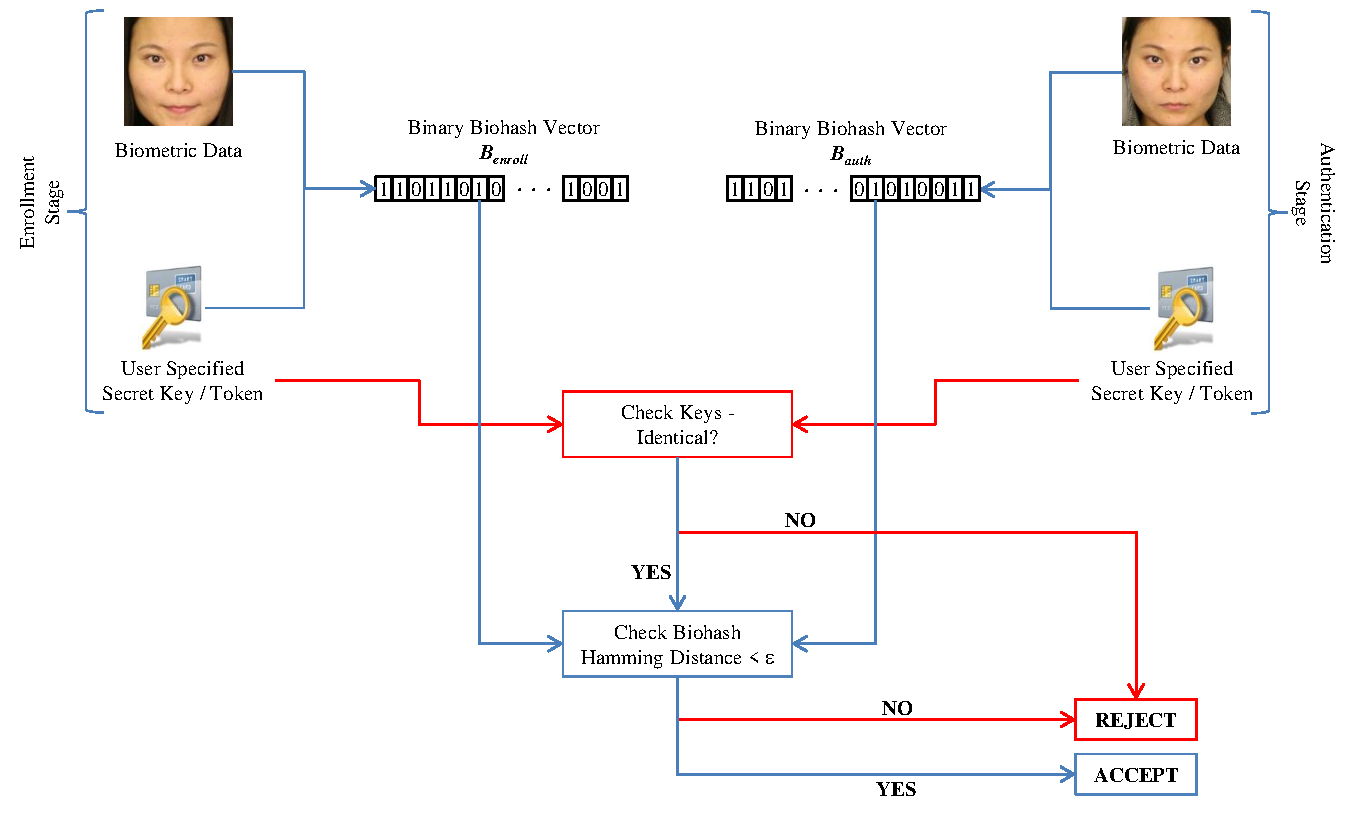
\includegraphics[width=0.7\linewidth]{figures/FIG1}
\caption{Illustration of biometric hashing-based verification.}
\label{fig2}
\end{center}
\end{figure*}

Biometric hashing (simply biohashing) schemes are simple yet
powerful biometric template protection methods~\cite{teoh2006, Bai, Karabat, Lumini, Rathgeb,Kuan}. Biohash is a binary and pseudo-random
representation of a biometric template and biometric hashing schemes
perform an automatic verification of a user based on his biohash (a
binary string). Two inputs of a biometric hashing scheme are: i)
biometric template and ii) user specific secret key. A biometric
feature vector is transformed into another space using a
pseudo-random set of vectors which are generated from the user's
secret key. Then, the result is binarized to produce a pseudo-random
bit-string which is called the biohash. The random projection matrix
is unique and specific to each user and it can be stored in a USB
token or a smartcard. In a practical system, a user specific random
matrix is calculated using a seed (a user specific secret key) that
is stored in a USB token or a smartcard microprocessor through a
pseudo random number generator. The seed is the same with that used
during the enrollment of a user and is different among different
users and different applications~\cite{teoh2006}. This allows
revocability of the subject's biohash in case it is compromised.
Also, the same biometric trait of a subject can be used in different
biometric recognition systems without constituting privacy threat as
two biohashes of the same person with different keys are unlinkable.

\subsubsection{Enrollment Stage}

The first stage in a biometric recognition system is the enrollment
stage in which a user is introduced to the system for the first
time. His biometric record is captured and converted to a
reference biometric template which will be compared to a fresh
sample at the authentication stage. This biometric template can be
stored either in a central database or a smart card that will be in
possession of the user.

\paragraph{Random Projection}

In the first step, a pseudo random projection (RP) matrix,
$\mathbf{R}\in\mathbb{R}^{k\times n}$, is generated to transform
the biometric feature vector of the user. The RP matrix elements are independent
and identically distributed (\textit{i.i.d}) and generated from a
Gaussian distribution with zero mean and unit variance by using a
Pseudo Random Number Generator (PRNG) with a seed derived from the
user's secret key. The RP matrix projects the feature vector onto
an $k$-dimensional space:

\begin{equation}
 \mathbf{y}=\mathbf{R}
 \mathbf{x},
\end{equation}
where $\mathbf{y}\in\mathbb{R}^{k\times1}$ is an intermediate
biohash vector.

\paragraph{Quantization (Binarization)}

In this step, elements of the intermediate biohash vector
$\mathbf{y}$ are binarized with respect to a threshold:

\begin{equation}
b_i = \begin{cases}
1, & y_i \geq \beta, \\
0, & \text{otherwise},
\end{cases}
\end{equation}
where $\mathbf{b}\in\ \left\{0,1\right\}^{k}$ denotes the biohash
vector of the user and $\beta$ denotes the quantization threshold
which can be 0 ($\text{sign}$ operator), the mean value of the
intermediate biohash vector $\mathbf{y}$ or any other pre-determined threshold depending on the system
design. After enrollment, biometric hashes are stored in a database or in a smart card.

\subsubsection{Authentication Stage}

During an authentication attempt, a claimer sends his biometric features
$\tilde{\textbf{x}}$ and secret key to the system. The system computes the claimer's test biometric hash
vector by using the same procedures in the enrollment phase. The
user is authenticated when the Hamming distance between
$\mathbf{b}_{enroll}$ (which denotes the biohash of the user
generated at the enrollment stage) and $\mathbf{b}_{auth}$ (which
denotes the biohash of the user generated at the authentication
stage) is below a pre-determined distance threshold $\epsilon$ as
follows:

\begin{equation}
\sum^{k}_{i=1}\mathbf{b}_{enroll}\left(i\right)\oplus\mathbf{b}_{auth}\left(i\right)\leq\epsilon
\end{equation}
where $\oplus$ denotes the binary XOR (exclusive OR) operator (Figure~\ref{fig2}).


\subsection{Homomorphic Encryption}

Homomorphic encryption concept enables the computation of overencrypted date without using the secret key. Although public-key encryption schemes that enable the performance of any kind of operations (fully homomorphic encryptions schemes) are proposed, they are still far from being used in real-life applications due to time and memory constraints. Therefore, partial homomorphic encryption cases are considered in this study.

A public-key encryption scheme \emph{Enc} is said to be additively homomorphic if there exists an efficient operantion $\odot$, not depending on the secret key, such that, for any pair of plain texts $x_1$ and $x_2$:

\begin{equation}
Enc(x_1)\odot Enc(x_2)\equiv Enc(x_1 + x_2).
\label{eqn4}
\end{equation}

The use of $\equiv$ means that the $\odot$ product of any pair of ciphertexts encrypting $x_1$ and $x_2$ is a ciphertext encrypting $x_1 + x_2$. An equality sign is not used since the encryption is randomized and many ciphertext encrypt the same plain text. For the sake of simplicity, we will use a $=$ symbol in the rest of this paper. Equation~\ref{eqn4} also implies that, with a multiplicative notation for $\odot$, for any message $x$ and integer $n$:

\begin{equation}
Enc(x)^n = Enc(n.x).
\label{eqn5}
\end{equation}

The most widely used additively homomorphic scheme, especially in the proposals for secure biometric identification, is the Paillier cryptosystems~\cite{Paillier99}. For a plain text message of $k$-bit long, Paillier ciphertexts are $2k$-bit long and $\odot$ operations are multiplications modulo a $2k$-bit integer. To ensure short-term security, $k$ must be at least 1024, which is equivalent to a 80-bit symmetric encryption or a 1024-bit RSA encrpytion~\cite{Bringer2013}.


\subsection{Biohashing via Homomorphic Encryption}

We assume that a biometric feature is represented by a vector $\mathbf{x}=[x_1, x_2, ..., x_i, ...]^T$ for $i=1,...,n$ (i.e. $\mathbf{x}\in\mathbb{R}^n$). Using the user specific random projection matrix $\mathbf{R}=[\mathbf{r}_1, \mathbf{r}_2, ..., \mathbf{r}_i, ...]^T$ for $i=1,...,k$ (i.e., $\mathbf{R}\in\mathbb{R}^{n\times k}$), input feature vector $\mathbf{x}$ is projected to the random space:

%\begin{equation}
%\mathbf{y} = \mathbf{R}\mathbf{x}\Rightarrow y_i=\mathbf{r}_i^T\mathbf{x}=r_{i1}x_1+r_{i2}x_2+...+r_{in}x_n.
%\label{eqn6}
%\end{equation}

\begin{align}
\mathbf{y}& =\mathbf{R}\mathbf{x}\\
y_i& =\mathbf{r}_i^T\mathbf{x}\\
&=r_{i1}x_1+r_{i2}x_2+...+r_{in}x_n.
\label{eqn6}
\end{align}

The client homomorphically encrypts each component of the feature vector and sends the obtained ciphertexts $Enc(x_1),...,Enc(x_n)$ to the server. Then using the encrypted components of $\mathbf{x}$, the server computes the encrypted components of the intermediate biohash vector $\mathbf{y}$ as follows:

%\begin{equation}
%Enc(y_i) = Enc(r_{i1}x_1)\times Enc(r_{i2}x_2)\times\ldots\times Enc(r_{in}x_n)
%\label{eqn7}
%\end{equation}

\begin{align}
Enc(y_i) &= Enc(r_{i1}x_1 + r_{i2}x_2 + \ldots + r_{in}x_n)\\
&= Enc(r_{i1}x_1)\times Enc(r_{i2}x_2)\times\ldots\times Enc(r_{in}x_n)\\
&=Enc(x_1)^{r_{i1}}\times Enc(x_2)^{r_{i2}}\times\ldots\times Enc(x_n)^{r_{in}}.
\label{eqn7}
\end{align}

Using the partial homomorphic properties, each encrypted component, $y_i$ is calculated in the encrypted domain and the encrypted intermediate biohash vector is obtained:

\begin{equation}
Enc(\mathbf{y}) = [Enc(y_1), Enc(y_2), \ldots, Enc(y_k)].
\label{eqn8}
\end{equation}

The next step is to compare each component of $\mathbf{y}$ with a threshold. If $y_i$ is greater than the threshold, corresponding bit of the biohash $b_i$ will be assigned to 1, otherwise, to 0.

\textcolor{red}{TAM OLARAK BU NOKTADA REAL VALUED $y_i$ ILE REAL VALUED THRESHOLDU KARSILASTIRIP BUYUKSE 1 KUCUKSE 0 OLARAK BIOHASHI OLUSTURACAGIZ.\\\\
BU KARSILAŞSTIRMA ISLEMINI $Enc(y_i) \gtrless Enc(THR)$ NASIL YAPACAGIMIZI BULMA NOKTASINDAYIZ.\\\\
EKLENECEKLER: BIOHASH PROTOKOL CIZIMI}

\begin{figure*}
\pseudocode{
\textbf{User} \<\< \textbf{System} \\[][\hline]
\\
\text{compute $\{Enc(x_i)$}:i=1,\ldots,n\} \<\< \\
\< \sendmessageright*{\text{$Enc(\mathbf{x})=[Enc(x_1), Enc(x_2),\ldots,Enc(x_n)]$}} \< \\
\<\< \text{compute \{$Enc(x_i)^{r_{ji}}: i=1,\ldots,n; j=1,\ldots,k$\}} \\
\<\< \text{$Enc(\mathbf{y})=[Enc(y_1), Enc(y_2),\ldots,Enc(y_k)]$} \\
\<\< \text{compute \{$Enc(y_i)\gtrless Enc(THR_i):i=1,\ldots,k$\}} \\
\<\< \text{$Enc(\mathbf{b})=[Enc(b_1), Enc(b_2),\ldots,Enc(b_k)]$} \\
\<\< \text{Save $Enc(\mathbf{b}_{enroll})$ to database} \\
\< \sendmessageleft*{\text{Response: Record saved to database}} \< \\
}
\caption{\textcolor{red}{Enrollment Flow (KABACA AKIS BU SEKILDE - TABI COK DAHA DETAYLI CIZERIZ)}}
\end{figure*}

\begin{figure*}
\pseudocode{
\textbf{User} \<\< \textbf{System} \\[][\hline]
\\
\text{compute $\{Enc(x_i)$}:i=1,\ldots,n\} \<\< \\
\< \sendmessageright*{\text{$Enc(\mathbf{x})=[Enc(x_1), Enc(x_2),\ldots,Enc(x_n)]$}} \< \\
\<\< \text{compute \{$Enc(x_i)^{r_{ji}}: i=1,\ldots,n; j=1,\ldots,k$\}} \\
\<\< \text{$Enc(\mathbf{y})=[Enc(y_1), Enc(y_2),\ldots,Enc(y_k)]$} \\
\<\< \text{compute \{$Enc(y_i)\gtrless Enc(THR_i):i=1,\ldots,k$\}} \\
\<\< \text{$Enc(\mathbf{b})=[Enc(b_1), Enc(b_2),\ldots,Enc(b_k)]$} \\
\\
\<\< \text{calculate Hamming Distance between} \\
\<\< \text{$Enc(\mathbf{b})$ and $Enc(\mathbf{b}_{enroll})$} \\
\< \sendmessageleft*{\text{Authentication Result: Yes / No}} \< \\
}
\caption{\textcolor{red}{Authentication Flow (KABACA AKIS BU SEKILDE - TABI COK DAHA DETAYLI CIZERIZ)}}
\end{figure*}


%\procedure{My Protocol}{
%\textbf{Alice} \> \> \textbf{Bob} \\
%}

%\p r o c e d u r e {My P r o t o c o l }{%
%\ t e x t b f { A l i c e } \> \> \ t e x t b f {Bob} \\
%b \samp le \ b in \> \> \\
%\> \ s e n dm e s s a g e r i g h t ∗{\ t e x t { s end o v e r } b} \> \\
%\> \> \ t e x t {do som eth ing } \\
%\> \ s e n dm e s s a g e l e f t ∗{\ t e x t { s end o v e r s t h . e l s e }} \> \\
%\ t e x t { f i n a l i z e } \> \> }




\section{Conclusion}
The conclusion goes here.




% conference papers do not normally have an appendix


% use section* for acknowledgement
\section*{Acknowledgment}


The authors would like to thank...





% trigger a \newpage just before the given reference
% number - used to balance the columns on the last page
% adjust value as needed - may need to be readjusted if
% the document is modified later
%\IEEEtriggeratref{8}
% The "triggered" command can be changed if desired:
%\IEEEtriggercmd{\enlargethispage{-5in}}

% references section

% can use a bibliography generated by BibTeX as a .bbl file
% BibTeX documentation can be easily obtained at:
% http://www.ctan.org/tex-archive/biblio/bibtex/contrib/doc/
% The IEEEtran BibTeX style support page is at:
% http://www.michaelshell.org/tex/ieeetran/bibtex/
%\bibliographystyle{IEEEtran}
% argument is your BibTeX string definitions and bibliography database(s)
%\bibliography{IEEEabrv,../bib/paper}
%
% <OR> manually copy in the resultant .bbl file
% set second argument of \begin to the number of references
% (used to reserve space for the reference number labels box)
%\begin{thebibliography}{1}
%
%\bibitem{Ferrer2002}
%Josep  Domingo-Ferrer.   A  provably  secure  additive  and  multiplicative
%privacy  homomorphism,\emph{Lecture  Notes  in  Computer  Science},  Volume 2433/2002:471–483, 2002
%\bibitem{Gentry2009}
%Craig Gentry.  Fully Homomorphic Encryption Using Ideal Lattices. \emph{41st ACM Symposium on Theory of Computing (STOC)},
%2009.
%\end{thebibliography}

\bibliographystyle{IEEEtran}
\bibliography{hmmBiohash}


% that's all folks
\end{document}


